\documentclass[journal,12pt,twocolumn]{IEEEtran}

\usepackage{setspace}
\usepackage{gensymb}
\usepackage[cmex10]{amsmath}
\usepackage{tikz}
\usetikzlibrary{automata,positioning}
\usepackage{amsthm}
\usepackage{amsmath}
\usepackage{blkarray}
\usepackage{mathrsfs}
\usepackage{mleftright}
\usepackage{txfonts}
\usepackage{stfloats}
\usepackage{bm}
\usepackage{cite}
\usepackage{cases}
\usepackage{subfig}
\usepackage{mathtools}  
\usepackage{xfrac} 
\usepackage{float}
\usepackage{flafter}
\usepackage{longtable}
\usepackage{multirow}

\usepackage{enumitem}
\usepackage{mathtools}
\usepackage{steinmetz}
\usepackage[english]{babel}
\usepackage[document]{ragged2e}

\usepackage{circuitikz}
\usepackage{verbatim}
\usepackage{tfrupee}
\usepackage[breaklinks=true]{hyperref}
\usepackage{graphicx}
\usepackage{tkz-euclide}

\usetikzlibrary{calc,math}
\usepackage{listings}
    \usepackage{color}                                            %%
    \usepackage{array}                                            %%
    \usepackage{longtable}                                        %%
    \usepackage{calc}                                             %%
    \usepackage{multirow}                                         %%
    \usepackage{hhline}                                           %%
    \usepackage{ifthen}                                           %%
    \usepackage{lscape}     
\usepackage{multicol}
\usepackage{chngcntr}

\DeclareMathOperator*{\Res}{Res}

\renewcommand\thesection{\arabic{section}}
\renewcommand\thesubsection{\thesection.\arabic{subsection}}
\renewcommand\thesubsubsection{\thesubsection.\arabic{subsubsection}}

\renewcommand\thesectiondis{\arabic{section}}
\renewcommand\thesubsectiondis{\thesectiondis.\arabic{subsection}}
\renewcommand\thesubsubsectiondis{\thesubsectiondis.\arabic{subsubsection}}


\newcommand{\define}{\stackrel{\triangle}{=}}


\theoremstyle{definition}
\newtheorem{definition}{Definition}[section]
\newtheorem{theorem}{Theorem}[section]
\newtheorem{lemma}[theorem]{Lemma}
\newtheorem*{remark}{Remark}

\bibliographystyle{IEEEtran}
\raggedbottom
\setlength{\parindent}{0pt}
\providecommand{\mbf}{\mathbf}
\providecommand{\pr}[1]{\ensuremath{\Pr\left(#1\right)}}
\providecommand{\qfunc}[1]{\ensuremath{Q\left(#1\right)}}
\providecommand{\sbrak}[1]{\ensuremath{{}\left[#1\right]}}
\providecommand{\lsbrak}[1]{\ensuremath{{}\left[#1\right.}}
\providecommand{\rsbrak}[1]{\ensuremath{{}\left.#1\right]}}
\providecommand{\brak}[1]{\ensuremath{\left(#1\right)}}
\providecommand{\lbrak}[1]{\ensuremath{\left(#1\right.}}
\providecommand{\rbrak}[1]{\ensuremath{\left.#1\right)}}
\providecommand{\cbrak}[1]{\ensuremath{\left\{#1\right\}}}
\providecommand{\lcbrak}[1]{\ensuremath{\left\{#1\right.}}
\providecommand{\rcbrak}[1]{\ensuremath{\left.#1\right\}}}

\newcommand{\sgn}{\mathop{\mathrm{sgn}}}
\providecommand{\abs}[1]{\vert#1\vert}
\providecommand{\res}[1]{\Res\displaylimits_{#1}} 
\providecommand{\norm}[1]{\lVert#1\rVert}
%\providecommand{\norm}[1]{\lVert#1\rVert}
\providecommand{\mtx}[1]{\mathbf{#1}}
\providecommand{\mean}[1]{E[ #1 ]}
\providecommand{\fourier}{\overset{\mathcal{F}}{ \rightleftharpoons}}
%\providecommand{\hilbert}{\overset{\mathcal{H}}{ \rightleftharpoons}}
\providecommand{\system}{\overset{\mathcal{H}}{ \longleftrightarrow}}
	%\newcommand{\solution}[2]{\textbf{Solution:}{#1}}
\newcommand{\solution}{\noindent \textbf{Solution: }}
\newcommand{\cosec}{\,\text{cosec}\,}
\providecommand{\dec}[2]{\ensuremath{\overset{#1}{\underset{#2}{\gtrless}}}}
\newcommand{\myvec}[1]{\ensuremath{\begin{pmatrix}#1\end{pmatrix}}}
\newcommand{\mydet}[1]{\ensuremath{\begin{vmatrix}#1\end{vmatrix}}}
\makeatletter
\@addtoreset{figure}{problem}
\makeatother
\let\StandardTheFigure\thefigure
\let\vec\mathbf
\renewcommand{\thefigure}{\theproblem}
\def\putbox#1#2#3{\makebox[0in][l]{\makebox[#1][l]{}\raisebox{\baselineskip}[0in][0in]{\raisebox{#2}[0in][0in]{#3}}}}
     \def\rightbox#1{\makebox[0in][r]{#1}}
     \def\centbox#1{\makebox[0in]{#1}}
     \def\topbox#1{\raisebox{-\baselineskip}[0in][0in]{#1}}
     \def\midbox#1{\raisebox{-0.5\baselineskip}[0in][0in]{#1}}

\lstset{
frame=single, 
breaklines=true,
columns=fullflexible
}
\begin{document}
\title{Assignment 3}
\author{Vibhavasu Pasumarti - EP20BTECH11015}
\maketitle
\newpage
\bigskip
\renewcommand{\thefigure}{\theenumi}
\renewcommand{\thetable}{\theenumi}
Download all python codes from 
\begin{lstlisting}
https://github.com/VIB2020/AI1103/blob/main/Assignment%203/code/Assignment%203.py
\end{lstlisting}
and latex-tikz codes from 
\begin{lstlisting}
https://github.com/VIB2020/AI1103/blob/main/Assignment%203/Assignment%203.pdf
\end{lstlisting}
\section{\large GATE 2015 (EE paper 01 new 2), Q 27 (Electrical Engg section)}
Two players A, and B alternately keep rolling a fair dice. The person to get a six first wins the game. Given that player A starts the game, the probability that A wins the game is:\\[5pt]
\begin{enumerate}[label=(\Alph*)]
    \item $\dfrac{5}{11}$\\
    \item $\dfrac{1}{2}$ \\
    \item $\dfrac{7}{13}$\\
    \item $\dfrac{6}{11}$
\end{enumerate}
\section{\Large Solution}
\begin{itemize}
    \item Given the die is fair.
    \item So, for any given throw by A or B:\\
    The probability of getting 6 = $\dfrac{1}{6}$ = p (say)\\
    The probability of NOT getting 6 = $\dfrac{5}{6}$ = q (say)
\end{itemize}
Constraint: A starts the game and A should win.\\
$\implies$ Until A wins, both A and B cannot win.\\
%$\implies$ B(State 2) is absorbing state and it represents the state A loses and B wins.\\
\begin{figure}[!htb]
Corresponding Markov chain is:\\
\begin{center}
    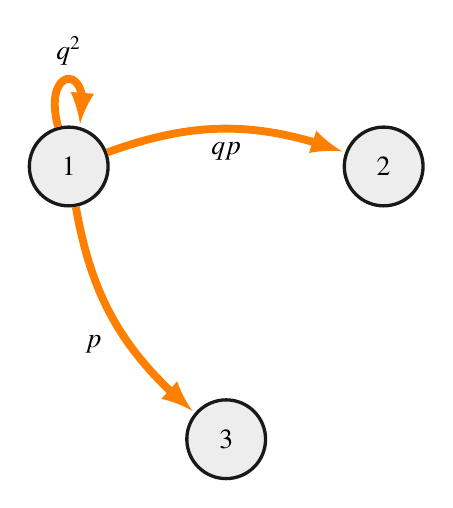
\begin{tikzpicture}[roundnode/.style={circle, draw=black!90, fill=black!7, very thick, minimum size=1cm}]
        \node [roundnode] at (0, 0)     (a)     {1};
        \node [roundnode] at (4, 0)     (b)     {2};
        \node [roundnode] at (2, -3.4641) (w) {3};
        \draw[every loop, auto=right, line width=1mm,
                >=latex, draw=orange,fill=orange]
            (a) edge[bend left=20] node {$qp$} (b)
            (a) edge[loop above=40] node {$q^2$} (a)
            (a) edge[bend right=20] node {$p$} (w);
    \end{tikzpicture}
%        \caption{Modified Markov chain}
        \label{fig:Fig1}
\end{center}
\end{figure}
\begin{table}[!htb]
    \begin{center}
    \begin{tabular}{|c|c|}
        \hline
        State & Corresponding description \\
        \hline
        1 & A and B both lose.\\
        \hline
        2 & A loses and B wins.\\
        \hline
        3 & WINNER\\
        \hline
      \multicolumn{2}{c}{Table 1: State description table}
    \end{tabular}
    \end{center}
\end{table}
\begin{definition}
    \vspace{2cm}
    2 and 3 are ABSORBING states.\\
    Transition/Stochastic matrix is: T\\
    \centering
         \text{\small (From)} \begin{blockarray}{ cccc }
                \multicolumn{3}{c}{(\small To)}\\
                & 1 & 2 & 3 \\
                \begin{block}{ c @{\quad} [ @{\,} *{3}{c} @{\,} ] }
                    1 & $q^2$ & qp & p\\ 
                    2 & 0 & 1 & 0\\
                    3 & 0 & 0 & 1\\
                \end{block}
           \end{blockarray} = T
\end{definition}
\begin{theorem}
Every transition matrix can be partitioned as $\mleft(
    \begin{array}{c|c}
        Q & P\\
        \hline
        O & J\\
    \end{array}
    \mright)$\\
    where Q arise from transition probabilities between non-absorbing states\\
    R arises from Transition probability from non-absorbing state to absorbing state.\\
    O = Null matrix,
    J = Identity matrix\\
    $T^k$ approaches $\overline{T}$ as k increases.
    $\overline{T}$ is the limiting matrix and
    $\overline{T} = \myvec{O & NP\\O & J}$\\
    where N is the fundamental matrix.
    $N = (I - Q)^{-1}$\\
    \end{theorem}
\begin{definition}
    The matrix D = NP gives the probability of ending up in the absorbing states (2 and 3) when the chain starts from a non-absorbent state 1.
\end{definition}
\begin{align}
    T = \mleft(
    \begin{array}{c| c c}
        q^2 & qp & p\\
        \hline
        0 & 1 & 0\\
        0 & 0 & 1\\
    \end{array}
    \mright)   \\ 
        Q = \myvec{q^2},
        P = \myvec{qp & p},
        O = \myvec{0 \\ 0},
        J = \myvec{1 & 0\\0 & 1} \label{eq:eqn1}
    \end{align}

    \begin{align}
        N = \myvec{1 - q^2}^{-1} = \myvec{\dfrac{1}{1-q^2}}\\
        D = NP = \myvec{\dfrac{qp}{1 - q^2} & \dfrac{p}{1 - q^2}}\\
        \pr{\text{A wins}} = D_2 = \dfrac{p}{1 - q^2} = \frac{\frac{1}{6}}{1 - \frac{25}{36}} = \dfrac{6}{11}
    \end{align}
        \centering
\[
    \pr{\text{A wins}} = \dfrac{6}{11}
\]
OPTION D is correct
\end{document}
